\documentclass[a4paper, 12pt]{article}
\usepackage[utf8]{inputenc}
\usepackage{geometry}
\usepackage{polski}
\usepackage{graphicx}
\usepackage{float}
\usepackage{etoolbox,refcount}
\usepackage{multicol}

\newgeometry{left=2cm, right=2cm, bottom=2cm, top=1.5cm}

\begin{document}
	\begin{figure}[H]
		\centering
		\includegraphics[height=6cm, width=\textwidth]{./grafika/lena.png}
	\end{figure}
	\section{Cel ćwiczenia}
		Celem ćwiczenia jest zapoznanie się z charakterystykami skokowymi regulatora PID z wyjściem ciągłym, poprzez opserwację ich przebiegów dla zadanych parametrów regulatora.
	\section{Schemat stanowiska}
		\begin{figure}[H]
			\centering
			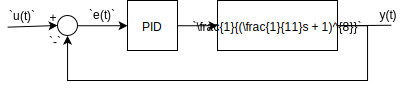
\includegraphics[width=\textwidth]{./grafika/schemat.png}
		\end{figure}
		Stanowisko składa się z szafy w której znajduje się regulator EFTRONIK X oraz z wyświetlaczy wartości zadanej i sterowanej. Do stanowiska należą trzy stacyjki ADS-31, jeden zadajnik \linebreak ADS-11, którego celem jest symulowanie skoku jednostkowego na układ. Zadaniem stacyjek ADS-31 jest wstępna polaryzacja, ustalenie poziomu zera oraz poziomu jedynki (odpowiednio 20\% i 70\% sygnału). Na szafie znajdowały się dwa przyciski, przy czym wciśnięcie jednego wypychało drugi - były odpowiedzialne za ustalanie pracy w trybie ciągłym lub w trybie dwupołożeniowym. Dodatkowo mieliśmy do układu podpięty oscyloskop, który pozwalał nam na akwizycję danych sygnału zadawanego na wyjściu regulatora.
	\section{Wstęp}
		Regulator EFTRONIK X pozwala na pracę na różnych warstwach, z których każda jest odpowiedzialna za inne jego funkcje jak i na różnych kanałach. Do naszych zastosowań wystarczająca była warstwa czwarta, która była odpowiedzialna za algorytmy regulacji. Pozostałe warstwy są odpowiedzialne za parametry generalne, wejścia analogowe, wejścia dyskretne, funkcje dwu zmiennych, wyjścia analogowe, wyjścia cyfrowe i za skalowanie wejść i wyjść analogowych.
		\newline
		\newline
		Regulator ten implementował algorytm PID ISA, co można było poznać po parametrach, jakie mieliśmy za zadanie ustawić. Głównym jego zadaniem jest usuwanie uchybu, który jest podany na wejście na poniższym układzie, a który się bierze ze sprzężenia zwrotnego w którym ten algorytm działa.
		\begin{figure}[H]
			\centering
			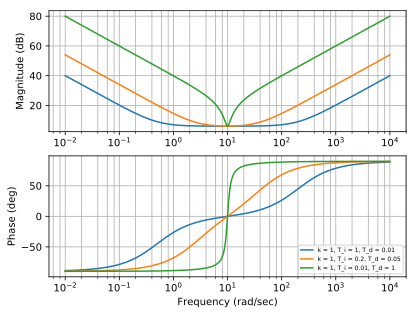
\includegraphics[width=0.5\textwidth]{./grafika/PID.png}
		\end{figure}
		Jednak na podstawie przebiegów można łatwo stwierdzić, że nie był to przypadek algorytmu PID idealnego, tylko rzeczywistego, którego transmitancja była dana wzorem:
		$$
		G(s) = k \cdot \left( 
		1 + \frac{1}{T_is} + \frac{T_ds}{Ts+1}
		\right)
		$$
		Przyjęliśmy tę formę zapisu rzeczywistego algorytmu PID, gdyż najbardziej przez to był trafiony człon różniczkujący i to jego działanie najbardziej odbiega od modelu matematycznego idealnego członu różniczkującego. 
		\newline
		\newline
		Poszczególne parametry odczytywaliśmy korzystając z przebiegów:
		\begin{itemize}
			\item $k$ - można poprowadzić prostą po części charakterystyki, która jest linią prostą. Z miejsca, gdzie miał miejsce skok można odczytać jej wartość
			\item $T_i$ - można ją odczytać na podstawie kąta nachylenia linii prostej w jaką zamienia się przebieg oraz odpowiednio manipulując wartością $k$.
			\item $T_d$ - można ją odczytać z zależności $U_{max} = k \left(1 + \frac{T_d}{T}\right)$, gdzie $U_max$ to maksimum przebiegu w chwili zadziałania akcji różniczkującej (pierwsze wybicie), a $T$ to różnica pomiędzy miejscem przecięcia się stycznej z osią, a czasem dla którego punkt miał miejsce.
		\end{itemize}
		Dla przypadku wyjścia dwupołożeniowego musieliśmy zastosować inne metody:
		\begin{itemize}
			\item $T_{imp}$ - czas impulsowania - różnica czasów między poszczególnymi załączeniami
			\item $T_i$ - można wyznaczyć na podstawie dwóch kolejnych przedziałów (oprócz pierwszego, bo działa tam różniczkowanie) $T_i = \frac{T^2_{imp}}{5(d_2-d_1)}$, gdzie $d_2$ i $d_1$ to czas trwania dwóch kolejnych przedziałów
			\item $k$ - można wyznaczyć przy pomocy liniowej ekstrapolacji wartość sygnału w chwili zerowej, a co za tym idzie też współczynnik wzmocnienia - analogicznie jak w ciągłym
			\item $T_d$ - nie udało się nam wyznaczyć, ze względu na zbyt duży czas impulsowania, występowanie stałej czasowej związanej z tym, że mieliśmy do czynienia z obiektem rzeczywistym oraz ze względu na przekraczanie przez sterowanie wartości maksymalnej. Oprócz tego zaistniały inne przyczyny, które zostały wyjaśnione we wnioskach.
		\end{itemize}
	\section{Przeprowadzenie ćwiczenia}
		Ćwiczenie rozpoczęliśmy od sprawdzenia w jakim stanie poprzednia grupa zostawiła stanowisko (np. czy regulator był pozostawiony w trybie ciągłym, czy dwupołożenieniowym oraz jego nastawy). Następnie przystąpiliśmy do sprawdzania w jakim stanie się znajdują poszczególne stacyjki. Upewniwszy się, że wszystko działa jak powinno, zapoznaliśmy się z działaniem danego modelu oscyloskopu, zdejmując charakterystykę próbną.
		\newline 
		\newline
		Ponieważ mieliśmy do czynienia z już wcześniej ustawionym regulatorem na wyjście ciągłe, rozpoczęliśmy właśnie od nich pomiary dla różnych wartości parametrów. Pomiary były zdejmowane z oscyloskopu i w razie błędnego pomiaru od razu kasowane przy pomocy laptopa.
		\newline
		\newline
		Następnie zmieniliśmy położenie przełącznika czerwony/niebieski na sterowanie z wyjściem dwupołożeniowym i zmieniliśmy też tryb pracy sterownika w odpowiedniej komórce pamięci. Po zmianie ustawień przystąpiliśmy do pomiarów charakterystyk regulatora dla kilku różnych konfiguracji. Ze względu na nieintuicyjne zachowanie sterownika w tym trybie mogliśmy niestety zatracić dużo informacji, zdejmując charakterystykę za późno z oscyloskopu (np. czas różniczkowania).
	\section{Pobrane dane}
		Osie pionowe są wyskalowane w woltach, a poziome w sekundach.
		\begin{figure}[H]
			\centering
			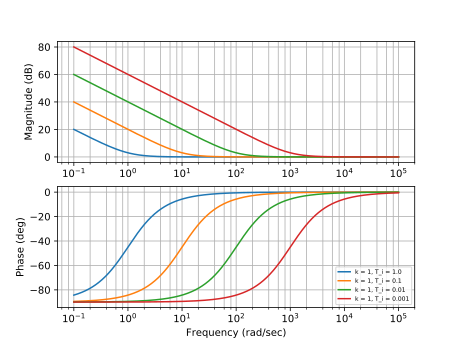
\includegraphics[width=0.9\textwidth]{./grafika/PI.png}
		\end{figure}
		Powyższy wykres przedstawia regulator PI.\newline 
		Jego parametry wprowadzone: $k = 1$, $T_i = 3$, $T_d = 0$
		\newline
		Parametry zmierzone:
		$k = 1$, $T_i = 2,9$
		\newline
		\newline
		Można na tym schemacie zauważyć, że mimo istnienia dobrej jakości członów proporcjonalnych i inercyjnych, dalej występuje duża inercja w układzie.
		\begin{figure}[H]
			\centering
			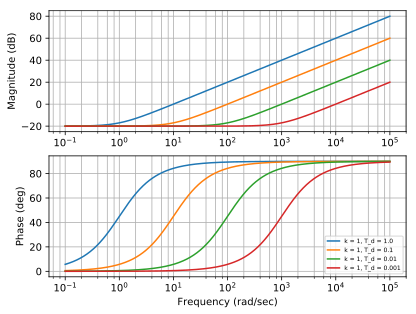
\includegraphics[width=0.9\textwidth]{./grafika/PD.png}
		\end{figure}
		Powyższy wykres przedstawia regulator PD. \newline
		Jego parametry wprowadzone: $k = 0,5$, $T_i = 0$, $T_d = 5$ \newline
		Jego parametry odczytane z wykresu: $k = 0,5$, $T_d = 4,8$
		\begin{figure}[H]
			\centering
			\includegraphics[width=0.9\textwidth]{./grafika/PIDI.png}
		\end{figure}
		Powyższy wykres przedstawia regulator PID. \newline
		Jego parametry wprowadzone: $k = 2$, $T_i = 5$, $T_d = 1$ \newline
		Jego parametry odczytane z wykresu: $k = 2,1$, $T_i = 5,5$ $T_d = 1,3$
		\newline
		Jest to przykład, kiedy element całkujący doprowadził do przekroczenia maksymalnej wartości sygnału.
		\newpage
		Dla przejrzystości przypadków, gdzie mamy do czynienia z wyjściem dwupołożeniowym zmieniliśmy oś na 0 i 1 aby zachować to co istotne na przebiegu. Osie czasu są w dalszym ciągu wyskalowane na 
		\begin{figure}[H]
			\centering
			\includegraphics[width=0.9\textwidth, height=6cm]{./grafika/cudo1.png}
		\end{figure}
		Parametry wprowadzone: $k = 1$, $T_i = 50$, $T_d = 1$, $T_{imp} = 10 $ \newline
		Wartości odczytane: $T_{imp} = 10$, $k = 1,1$, $T_i = 46$
		\begin{figure}[H]
			\centering
			\includegraphics[width=0.9\textwidth, height=6cm]{./grafika/cudo2.png}
		\end{figure}
		Parametry wprowadzone: $k = 2$, $T_i = 20$, $T_d = 1$, $T_{imp} = 5 $ \newline
		Wartości odczytane: $T_{5} = 10$, $k = 2,3$, $T_i = 18,2$ \newline
		
		Na powyższym przykładzie można bardzo dobrze zauważyć \ co się dzieje jak połączy się człon całkujący z małym czasem trwania impulsu - powoli cały czas impulsu jest przeznaczany na sygnał, następuje przepełnienie.
	\section{Wnioski}
		Na podstawie przebiegów odpowiedzi skokowych możemy zauważyć, że zgodnie z przewidywaniami modelu matematycznego, o którym dowiedzieliśmy się na wykładach, akcja różniczkująca regulatora odgrywa największą rolę w chwili dużych zmian wartości, jakie mają miejsce w początkowej fazie skoku jednostkowego. Akcja całkująca zyskuje na znaczeniu w późniejszych chwilach regulacji, a człon proporcjonalny pracuje ciągle na tym samym poziomie.
		\newline
		\newline
		Ćwiczenie zapoznało nas z kolejnym minimalistycznym interfejsem użytkownika, aczkolwiek o wiele bardziej przyjaznym niż ten z którym zetknęliśmy się w ćwiczeniu drugim. Wady, tamtego interfejsu znacznie wydłużały nam tamto ćwiczenie, te jednak pozwoliło nam na o wiele szybsze i płynniejsze poruszanie się pomiędzy odpowiednimi nastawami bez obaw o to, że sprawdzając adresy w dokumentacji pod którymi się znajdują regulator przejdzie w tryb podglądu, zmuszając nas do ponownego przeszukiwania wszystkich kolejnych opcji.
		\newline
		\newline
		Zapoznaliśmy się tu z kolejnym modelem oscyloskopu oraz z oprogramowaniem, które pozwala na odczyt zebranych z niego danych. Ze względu na obycie się ze sprzętem tego typu w trakcie laboratoriów z innych przedmiotów, nie mieliśmy problemu ani z pobieraniem danych na pamięć zewnętrzną USB, ani z dobieraniem parametrów ekranu oscyloskopu. Jedynym, co nam sprawiło problem był brak możliwości otworzenia niektórych pomiarów przy pomocy oprogramowania, gdyż otrzymywaliśmy poniższy komunikat błędu:
		\begin{figure}[H]
			\centering
			\includegraphics[width=\textwidth]{./grafika/error.png}
		\end{figure}
		Nie wiemy co mogło być powodem tego błędu, ale jest on powodem dla którego mamy mniej charakterystyk niż zamierzaliśmy początkowo przeanalizować. Błąd ten pojawił się dla późniejszych pomiarów, których dokonywaliśmy już dla charakterystyk regulatora PID z wyjściem dwupołożeniowym.
		\newline
		\newline
		Mogliśmy zaobserwować tu odpowiedzi wygenerowane przez rzeczywisty sterownik PID, można to zauważyć po sposobie w jaki sterowanie opada po zakończeniu działania akcji różniczkującej w przypadku algorytmu PID ciągłego. To jak akcja całkująca szybko przekracza maksymalną wartość napięcia pokazało nam dlaczego algorytm PID jest realizowany w pętli sprzężenia zwrotnego - gdyż w innym przypadku doszłoby bardzo szybko do ścięcia sygnału przez osiągnięcie jego maksymalnej wartości. Na przebiegach można również zaobserwować szumy, które raz zaniżają nieco wartość, a innym razem zawyżają, jednak zawsze o wartość na tyle małą, że nie przeszkadza w działaniu regulatora.
\end{document}